\subsection{Tracking Vehicles}
\label{sec:tracking}

In order to achieve the goals of the system, vehicle counting and speed estimation, it is necessary to keep track of the vehicles in the scene. This means knowing how the detected blobs relate to each other between consecutive frames.\\

\noindent For this purpose, we assume a Linear Dynamics Model (LDM) and, consequently, a Kalman filter \cite{kalman} is used for tracking. Under this framework, the state of each vehicle is supposed to vary linearly on each time step and suffer a slight perturbation (with Gaussian distribution). Similarly, the detection obtained is supposed to be a linear transformation of the previous state, plus some Gaussian noise as well. The procedure consists of making a prediction of the object's next state, based on all the previous measurements, and once the new detection is done, update this prediction. The equations derived by the Kalman filter are the optimal ones in the case of an LDM.\\

\noindent The assumption of a linear model is not so restrictive as it may seem. This can handle, for instance, the projection (into the camera plane) of the movement of cars traveling at a constant speed. In almost any road it is possible to find sectors with this characteristics. A 50 meter long straight part of the road would be enough for our system to work. Fig. \ref{fig:kalman} shows an example of kalman tracking for 2 vehicle in our sequence.

\begin{figure}[h]
\centering
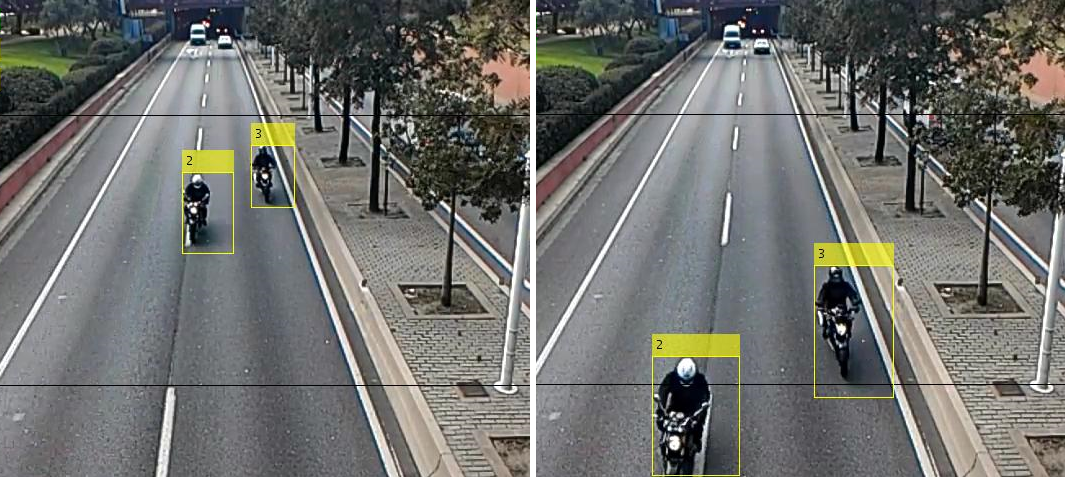
\includegraphics[width=240pt, height=130pt]{figures/example_kalman.png}
\caption{Sample of Kalman tracking detection for two vehicles along different frames.}
\label{fig:kalman}
\end{figure}